%!TeX program = xelatex
\documentclass[11pt]{article}

\usepackage{graphicx}
\usepackage{fancyhdr}
\usepackage{geometry}
\usepackage[utf8]{inputenc}
\usepackage{enumitem}
\usepackage{amsmath} 
\usepackage{multirow}
\usepackage{caption}
\usepackage{float}
\usepackage{fontspec}
\usepackage{cite}
\usepackage{listings}
%\setmainfont{UT Sans}
\usepackage{geometry}
\usepackage{xcolor}

\lstdefinestyle{customc}{
	belowcaptionskip=1\baselineskip,
	breaklines=true,
	frame=L,
	xleftmargin=\parindent,
	language=C,
	showstringspaces=false,
	basicstyle=\large\ttfamily,
	keywordstyle=\bfseries\color{green!40!black},
	commentstyle=\itshape\color{purple!40!black},
	identifierstyle=\color{blue},
	stringstyle=\color{orange},
}

\lstset{escapechar=@,style=customc}

\geometry{a4paper,left=20mm,right=20mm,total={160mm,220mm}}
\pagestyle{fancy}
\thispagestyle{plain}
\fancyheadoffset{0cm}
\rhead{\textit{Andrei Vasilcoi}\\Grupa 4452}

\renewcommand*\contentsname{Cuprins}
\renewcommand*\tablename{Tab.}
\renewcommand*\figurename{Fig.}
\renewcommand\refname{Bibliografie}
\renewcommand{\theenumi}{\Alph{enumi}}
\author{Andrei Vasilcoi}
\newcommand{\EqRow}{\vspace{1.5mm}}
\begin{document}
\begin{titlepage}

\newcommand{\HRule}{\rule{\linewidth}{0.5mm}}
	
\begin{center}
	%autor si indrumator mai jos
\textsc{\LARGE Universitatea Transilvania din Brașov}\\[0.5cm]

\includegraphics[width=0.25\textwidth]{logo_ut.jpg}\\[0.5cm]
\textsc{\Large Facultatea de Inginerie Electrică și Știința Calculatoarelor}\\[0.5cm]
\textsc{\large Departament Automatică și Informatică Aplicată}\\[1.5cm]
\HRule\\[0.5cm]
{\Large Proiect \textit{Ingineria reglării automate}}\\[0.5cm]
{\LARGE\bfseries Tema nr. 57}\\[0.5cm]
\HRule\\[2.5cm]
\begin{minipage}{1\textwidth}
	\begin{flushleft}
		\large
		\textit{Autor}\\
		Andrei \textsc{Vasilcoi}\\
	\end{flushleft}
\end{minipage}
~
\end{center}
\centering
\vspace{5cm}
{\large Iunie 2018, Brașov}\\[5cm]
\end{titlepage}

\newpage
\pagenumbering{arabic}
\tableofcontents

\newpage	
\section{Tema proiectului}
Se consideră un proces modelat prin funcția de transfer:
\EqRow
\begin{equation} 
G_p(s)=\frac{K_p}{(sT_{p1}+1)(sT_{p2}+1)(sT_{p3}+1)}
\EqRow
\end{equation}
Se cere să se realizeze o analiză comparativă a mai multor soluții privind proiectarea unui sistem de reglare automată care să respecte performanțele impuse: $e_{st}=0$, $M_v<=m_{v,max}$ și $t_s<=t_{s,max}$. (Valorile impuse ale indicatorilor de performanță sunt date în tabel.) Pentru notarea timpului de stabilire se consideră banda de stabilitate de 2\%. \\
Soluțiile impuse sunt:
\begin{enumerate}[label=\alph*)]
	\item proiectarea unui regulator PID prin metode de cvasi-optim: criteriul modulului standard sau varianta Kessler;
	\item metode experimentale de proiectare a regulatoarelor PID: metoda Ziegler-Nichols (a răspunsului la intrare treaptă);
	\item proiectarea unui sistem de reglare după stare.
\end{enumerate}
Detalii privind cerințele:
\begin{enumerate}[label=\arabic*.]
	\item Pentru fiecare soluție se vor realiza scheme Simulink și se vor nota performanțele obținute. Dacă este necesar, se vor ajusta suplimentar parametrii regulatoarelor până când sistemul de reglare respectă performanțele impuse.
	\item Pentru fiecare lege de reglare obținută se vor determina ecuațiile cu diferențe necesare unei implementări numerice. Se va prezenta codul sursă al unui program de implementare a cel puțin unui regulator.
	\item În capitolul de concluzii se va prezenta o comparație a performanțelor obținute, a efortului de proiectare și a altor aspecte considerate importante cu scopul de a argumenta alegerea unei soluții ca fiind cea mai potrivită pentru cazul considerat.
\end{enumerate}

\begin{center}
\captionof{table}{Date de proiectare}
\begin{tabular}{|c|c|c|c|c|c|c|c|}
	\hline
	{\multirow{2}{*}{Tema nr.} } &  \multicolumn{4}{ c| }{Parametrii procesului} & {\multirow{2}{*}{$M_{v, max}$}} & {\multirow{2}{*}{$t_{s, max}$}} & {\multirow{2}{*}{Student}} \\ \cline{2-5}
	&$K_p$ & $T_{p1}$ & $T_{p2}$ & $T_{p3}$ & & & \\ 
	\hline
 \multirow{2}*{57} & \multirow{2}*{1.1} & \multirow{2}*{0.7} & \multirow{2}*{0.5} & \multirow{2}*{10} & \multirow{2}*{1\%} & \multirow{2}*{3s} & \multirow{2}*{Vasilcoi S. Andrei} \\ &&&&&&& \\
	\hline
\end{tabular}
\end{center}

\section{Indicații și recomandări}
\begin{enumerate}[label=\alph*)]
	\item Pentru proiectarea prin metode analitice (de cvasi-optim), la determinarea prin calcul a parametrilor regulatorului se vor considera modele simplificate ale procesului dat. Simplificările trebuie să fie argumentate. La simulări însă, se va utiliza funcția de transfer dată inițial.
	\item Pentru metoda experimentală, este necesară o procesare cât mai precisă a răspunsului procesului în circuit deschis la semnal de intrare de tip treaptă. Pentru acest lucru este indicat să se realizeze un program Matlab.
	\item Pentru proiectarea unui sistem de reglare după stare, se va determina inițial modelul în spațiul stărilor. Apoi se va evalua controlabilitatea și observabilitatea modelului obținut.
	\item La determinarea ecuațiilor cu diferențe, valoarea aleasă a perioadei de eșantionare se va argumenta.
\end{enumerate}
\newpage
\section{Rezolvare}
\subsection{Proiectarea unui regulator PID prin metode de cvasi-optim: varianta Kessler}
Se consideră funcția de transfer:
\EqRow
\begin{equation}
G_p(s)=\frac{1.1}{(0.7s+1)(0.5s+1)(10s+1)}
\EqRow
\end{equation}
Se poate obseva că funcția de transfer a procesului nu are zerouri și are o  constantă de timp mare și două constante de timp mici, ce pot fi compensate. Pentru proiectarea regulatorului vom folosi criteriul modulului varianta Kessler. Varianta Kessler permite ca toate constantele de timp mici să fie înlocuite cu o singură constantă de timp obținută din suma acestora notată cu $T_{\Sigma}=T_{p1}+T_{p2}$.
Forma funcției de transfer în buclă deschisă pentru metoda Kessler este:
\vfill
\begin{equation} 
G_d^{CMVK}(s)=\frac{1}{2sT_{\Sigma}(sT_{\Sigma}+1)}
\end{equation}
\EqRow
\begin{equation} 
G_d^{CMVK}(s)=G_R(s)G_p(s)
\EqRow
\end{equation}
Pentru rezolvarea prin metoda Kessler calculele se vor efectua utilizând forma simplificată a procesului. În simulare însă se va folosi forma originală a procesului. Rezolvarea ecuațiilor și aflarea funcției de transfer a regulatorului este:
\vfill
$$T_{\Sigma}=0.7+0.5=1.2$$
\vfill
$$G_R(s)=\cfrac{G_d^{CMVK}(s)}{G_p(s)}=\cfrac{\cfrac{1}{2.4s(1.2s+1)}}{\cfrac{1.1}{(1.2s+1)(10s+1)}}=\cfrac{10s+1}{2.64s}=\cfrac{10}{2.64}\cfrac{10s+1}{10s}=3.78(1+\cfrac{1}{10s})\EqRow$$
Din rezolvare rezultă un regulator PI care are un zero ce compensează constanta de timp mare a procesului. De asemenea conține și componentă integrativă care asigură $e_{st}=0$. Funcția de transfer respectă condiția de realizabilitate fizică. Performanțele sistemului și identificarea coeficienților se pot observa în tabelul 2, Fig.1 și Fig.2.:
\begin{figure}[H]
	\centering
	\begin{minipage}{.4\textwidth}
		\centering
		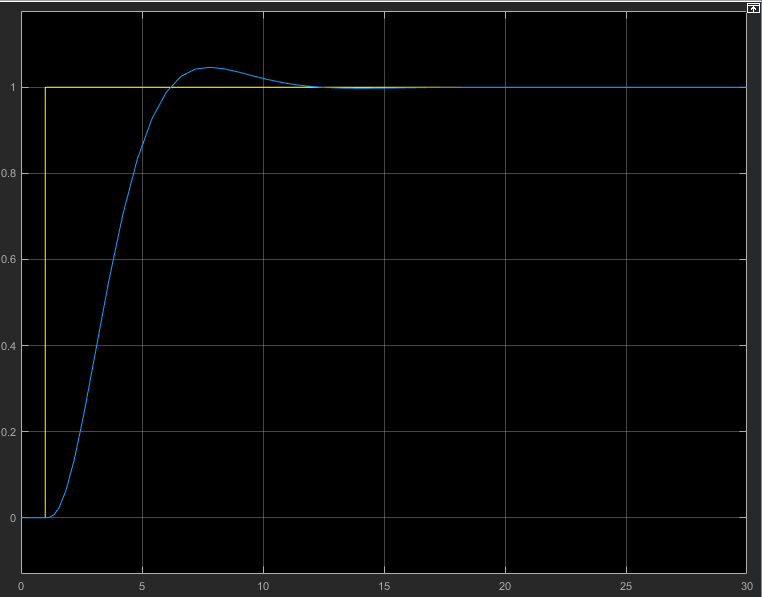
\includegraphics[width=.9\linewidth]{CMVK.png}
		\captionof{figure}{Răspunsul sistemului la intrare treaptă unitară}
		\label{fig:test1}
	\end{minipage}%
	\begin{minipage}{.6\textwidth}
		\centering
		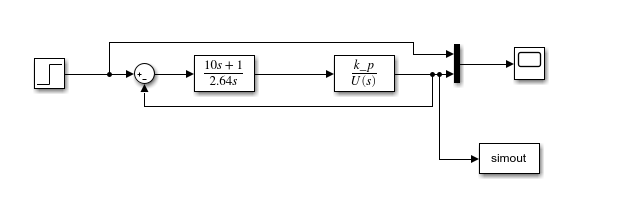
\includegraphics[width=.9\linewidth]{sim_cmvk.png}
		\captionof{figure}{Modelarea procesului în Simulink}
		\label{fig:test2}
	\end{minipage}
\end{figure}
\begin{center}
	\captionof{table}{Performanțe folosind varianta Kessler}
	\begin{tabular}{|c|c|c|c|c|c|c|}
		\hline
		&$e_{st}$&$M_v$&$t_s$&$K_r$&$T_i$\\
		\hline
		Impus&0&1&3&-&-\\
		\hline
		Obtinut&0&4.56&9.04&3.78&10\\
		\hline
	\end{tabular}
\end{center}
Având în vedere lucrarea experimentală 2 unde s-au observat efectele modificării parametrilor regulatorului asupra indicatorilor de calitate, s-a încercat atingerea performanțelor impuse prin încercări.
Pentru implementarea prin încercări s-a pornit de la următoarea formă a regulatorului PID prezentă în lucrarea 6:
\begin{equation} 
G_r(s)=k_r(1+\frac{1}{sT_i}+\frac{sT_d}{sT_f+1})
\end{equation}
Folosind modelul Simulink din Fig.3.
După ulterioare încercări de a modifica coeficienții regulatorului s-au obținut performanțele din Tab. 3 si Fig.3:
\EqRow
\begin{figure}[H]
	\centering
	\begin{minipage}{.4\textwidth}
		\centering
		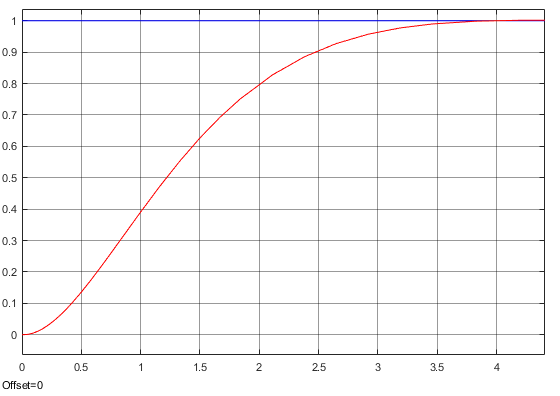
\includegraphics[width=1\linewidth]{incercari.png}
		\captionof{figure}{Răspunsul celui mai performant sistem din încercări}
		\label{fig:test2}
	\end{minipage}
	\begin{minipage}{.5\textwidth}
		\centering
		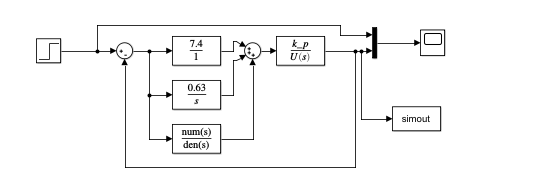
\includegraphics[width=1\linewidth]{sim_incercari.png}
		\captionof{figure}{Model PID folosit pentru încercări}
		\label{fig:test2}
	\end{minipage}
\end{figure}
\begin{center}
	\captionof{table}{Încercări experimentale}
	\begin{tabular}{|c|c|c|c|c|c|c|c|}
		\hline
		&$e_{st}$&$M_v$&$t_s$&$K_r$&$T_i$&$T_d$\\
		\hline
		Impus&0&1&3&-&-&-\\
		\hline
		Obținut&0&0.06&3.89&7&10&0.8\\
		Obținut&0&0.19&3.3&7.3&11&0.7\\
		Obținut&0&0.09&3.2&7.4&11.6&0.67\\
		\hline
	\end{tabular}
\end{center}
\EqRow
Pentru implementarea numerică a unui regulator trebuie determinată ecuația cu diferențe a acestuia.
Se pornește pentru prima implementare de la funcția de transfer a regulatorului PI obținut prin varianta Kessler:
$$G_r(s)=\cfrac{10s+1}{2.64s}\EqRow$$
Se obține $G(z^{-1})$ făcând substituția:
$$s=\frac{1-z^{-1}}{T_e}\EqRow$$

Unde $T_e$ reprezintă timpul de eșantionare. Acesta trebuie ales conform regulii lui Shannon: de 2 ori mai mic decât cea mai mică constantă de timp din funcția de transfer a procesului, în acest caz a regulatorului. De obicei se alege de până la 10 ori mai mică.\\
Considerând $T_e=0.1$, se obține:
$$G_r(z^{-1})=\frac{3.78z^{-1}-3.81}{z^{-1}-1}$$
Se aduce funcția la forma $G(q^{-1})$, unde $q^{-1}$ reprezintă operatorul de întârziere cu o unitate de timp $T_e$.
Pentru asta, se face substituția $z^{-1}=q^{-1}$.
$$G_r(q^{-1})=\frac{3.78q^{-1}-3.81}{q^{-1}-1}=\frac{u[k]}{e[k]}$$
Făcând înmulțirile pe diagonală, se obține:
$$q^{-1}u[k]-u[k]=3.78q^{-1}e[k]-3.81e[k]$$
Operatorul de întârziere este definit astfel: $q^{-n}y[k]=y[k-n]$. Folosind această proprietate obținem ecuația cu diferente a regulatorului:
$$u[k]=-3.78e[k-1]+3.81e[k]+u[k-1]$$

Pentru că răspunsul regulatorului PID cu parametrii obținuți prin încercări respectă performanțele impuse, pe lângă determinarea ecuațiilor cu diferențe pentru regulator, vom realiza și o implementare pentru un microcontroller.
Ecuația cu diferențe se obține aplicând aceeași metodă ca cea folosită anterior.
\begin{align}
G_r(s)&=\cfrac{58.31s^2+85.914s+7.4}{0.116s^2+11.6s}\notag\\
\notag\\
G_r(z^{-1})&=\cfrac{45.66z^{-2}+98.1z^{-1}+52.49}{0.09z^{-2}-1.09z^{-1}+1}\notag\\
\notag\\
G_r(q^{-1})&=\cfrac{45.66q^{-2}+98.1q^{-1}+52.49}{0.09q^{-2}-1.09q^{-1}+1}=\frac{u[k]}{e[k]}\notag
\end{align}
\begin{align}
0.09q^{-2}u[k]-1.09q^{-1}u[k]+u[k]=45.66q^{-2}e[k]+98.1q^{-1}e[k]+52.49e[k]\notag\\
\notag\\
u[k]=45.66e[k-2]+98.1e[k-1]+52.49e[k]-0.09u[k-2]+1.09u[k-1]\notag
\end{align}
\newpage
\begin{lstlisting}
float r = 1.f;

const int k = 2;
float last_u[k]={0,0,0};
float last_e[k]={0,0,0};

float update()
{
	//e[k]
	const float e = r - y;
	
	//u[k]=45.66e[k-2]+98.1e[k-1]+52.49e[k]-0.09u[k-2]+1.09u[k-1]
	const float u = 45.66f * last_e[k-2] + 98.1f * 
	last_e[k-1] + 52.49 * e - 0.09 * last_u[k-2] + 1.09 * last_u[k-1];
	
	for(int index = 1;index<k;index++)
	{
		last_u[index-1]=last_u[index];
		last_e[index-1]=last_e[index];
	}
	last_u[k-1]=u;
	last_e[k-1]=e;
	return u;
}

//intrerupere timer
ISR (TIMERx_OVF_vect)
{
	//citeste marimea de iesire
	//const float y = read();
	
	//trimite comanda
	//write(,update(y))
}
void setup()
{
	//setare timer cu intrerupere la t_e = 0.1
}
\end{lstlisting}

\newpage
\subsection{Metode experimentale de proiectare a regulatoarelor PID: metoda Ziegler-Nichols}
Pentru a aplica metoda experimentală este nevoie ca prima oară să se înregistreze valoarea răspunsului sistemului in buclă deschisă la mărimea de intrare treaptă unitară.\\
\begin{figure}[H]
	\centering
	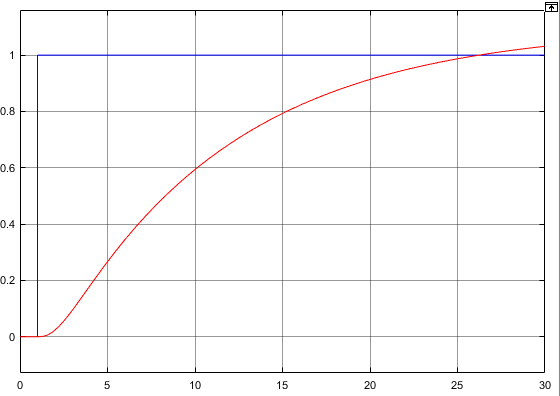
\includegraphics[width=.35\linewidth]{zn_desc.png}
	\captionof{figure}{Răspunsul sistemului în buclă deschisă}
	\label{fig:test2}
\end{figure}
Având aceste date putem calcula derivata de ordinul I. În continuare se va calcula punctul de maxim al derivatei de ordinul I si se va verifica în datele derivatei de ordinul II dacă punctul de maxim îndeplinește condițiile de a fi punct de inflexiune.
O dată găsit acest punct de inflexiune se va trasa tangenta la graficul răspunsului sistemului prin punctul de inflexiune. Se găsesc punctele de intersecție cu axele $x$ și $y$. \\
\begin{figure}[H]
	\centering
	\begin{minipage}{.5\textwidth}
		\centering
		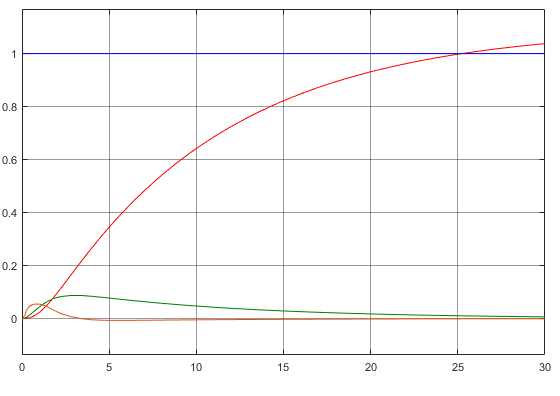
\includegraphics[width=.9\linewidth]{zn_pr.png}
		\captionof{figure}{Răspunsul sistemului și derivatele de ordin I și II}
		\label{fig:test1}
	\end{minipage}%
	\begin{minipage}{.6\textwidth}
		\centering
		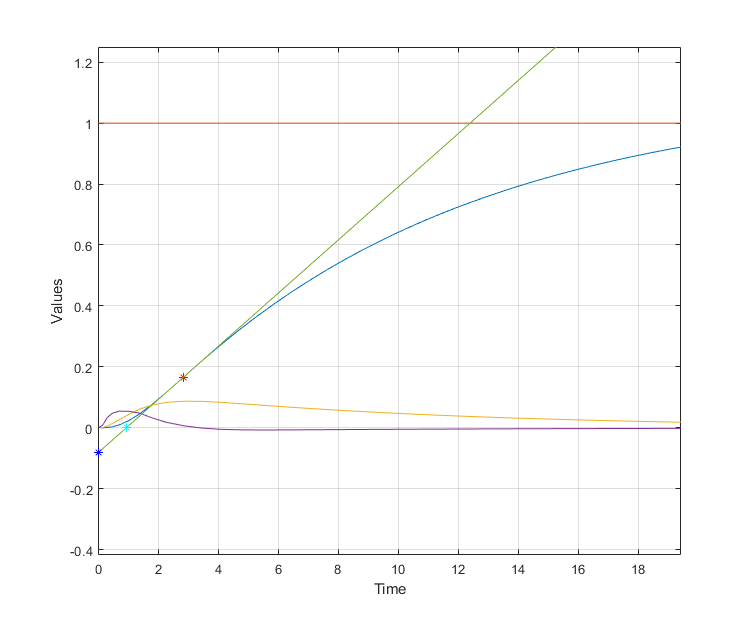
\includegraphics[width=.9\linewidth]{zn_pct.png}
		\captionof{figure}{Puncte necesare pentru proiectare}
		\label{fig:test2}
	\end{minipage}
\end{figure}
Aceste puncte de intersecție semnifică valorile $a$ și $L$ din algoritmul metodei experimentale care se vor folosi pentru a obține valorile estimate ale coeficienților regulatorului după cum urmează: 
\newpage
\begin{center}
	\captionof{table}{Formule prezente în curs pentru metoda Ziegler-Nichols}
	\begin{tabular}{|c|c|c|c|c|c|}
		\hline
		Regulator&$K_{r}$&$T_i$&$T_d$&$T_0$\\
		\hline
		P&$1/a$&-&-&$4L$\\
		\hline
		PI&$0.9/a$&$3L$&-&$5.7L$\\
		\hline
		PID&$1.2/a$&$2L$&$L/2$&$3.4L$\\
		\hline
	\end{tabular}
\end{center}
Valorile parametrilor $a$ și $L$ sunt:\\
$a=0.08\\
L=1.925$\\
La implementarea regulatorului se observă următoarele performanțe:
\begin{center}
	\captionof{table}{Performanțele folosind regulatorul proiectat prin metoda Ziegler-Nichols}
	\begin{tabular}{|c|c|c|c|c|c|c|}
		\hline
		&$e_{st}$&$M_v$&$t_s$&$K_r$&$T_i$&$T_d$\\
		\hline
		Impus&0&1&3&-&-&-\\
		\hline
		Obținut P&7&40&13&12.45&-&-\\
		\hline
		Obținut PI&0&50&16.05&11.2&5.77&-\\
		\hline
		Obținut PID&0&10&8.5&14.9&3.85&0.96\\
		\hline
	\end{tabular}
\end{center}
\begin{figure}[H]
	\centering
	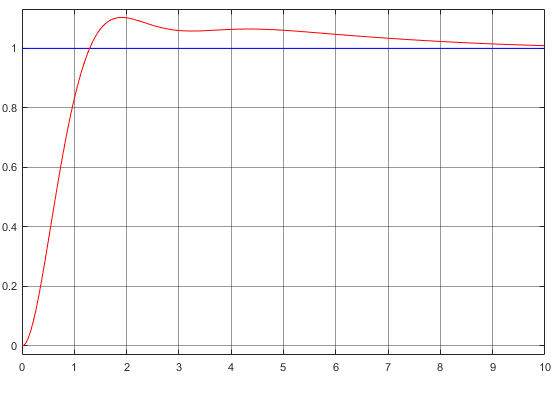
\includegraphics[width=.55\linewidth]{ZN.png}
	\captionof{figure}{Răspunsul sistemului folosind regulatorul PID proiectat prin metoda Ziegler-Nichols}
	\label{fig:test2}
\end{figure}
\newpage
\subsection{Proiectarea unui sistem de reglare după stare}
Proiectarea regulatorului după stare folosește metoda plasării polilor. Pentru ca această metodă să poată fi
folosită, sistemul trebuie să fie controlabil și observabil.
Considerăm sistemul de reglare modelat la stare conform ecuației matriceale:
\begin{align}
\dot{x}(t)&=Ax(t)+Bu(t)\\
y(t)&=Cx(t)
\end{align}
Unde $x(t)$ este vectorul n-dimensional de stare, $u(t)$ constituie semnalul de comandă (intrare), care este un
scalar, $A$ este marticea de stare de dimensiune $n \times n$ cu coeficienți constanți, $B$ reprezintă vectorul de intrare
cu dimensiunea $n \times 1$, iar $C$ este matricea de ieșire.
Pentru transformarea în spațiul stărilor s-a folosit funcția din Matlab $tf2ss$. \\
Sistemul curent are matricile:
\[A=
\begin{bmatrix}
-3.52       & -3.2 & -0.28\\
1       & 0 & 0\\
0      & 1 & 0\\
\end{bmatrix},
B=
\begin{bmatrix}
1 \\ 
0 \\
0 \\
\end{bmatrix},
C=\begin{bmatrix}
0  &0&0.31      \\
\end{bmatrix}
\]
Pentru că sistemul curent modelat nu are integrator, se va folosi reglarea combinată la stare cu regulator de
eroare de tip I.
Sistemul are funcționarea descrisă de ecuațiile (6) și (7), și
\begin{align}
u(t)&=-Kx(t)+k_{i}z(t)\\
\dot{z}(t)&=r(t)-y(t)=r(t)-Cx(t)
\end{align}
Metoda presupune aflarea matricei $K=(k_1 k_2 ... k_n)$, pentru un set de poli aleși
$-\mu_1, -\mu_2, ..., -\mu_n$. Polinomul caracteristic dorit, care realizează performanțele impuse, este:
\begin{equation}
c(s)=(s+\mu_1)(s+\mu_2)(s+\mu_3) ... (s+\mu_n)=s^n+\alpha_1s^{n-1}+\alpha_2s^{n-2}+...+\alpha_n
\end{equation}
Pe de altă parte, polinomul caracteristic al sistemului cu reacție la stare este:
\begin{equation}
c(s)=\det[sI-A+BK]=s^n+\beta_1s^{n-1}+\beta_2s^{n-2}+...+\beta_n
\end{equation}
Pentru identificarea valorilor matricei K se face corespondeța între coeficienții celor două polinoame:
\begin{align}
\alpha_1&=\beta_1\notag\\
\alpha_2&=\beta_2\notag\\
&\vdots\notag\\
\alpha_n&=\beta_n\notag
\end{align}

Înainte de a determina matricea K, trebuie să se verifice dacă sistemul este controlabil și observabil.\\
Controlabilitatea se referă la posibilitatea de a ghida sistemul dintr-o stare inițială $x$ spre origine, într-un timp finit, prin intermediul unei intrări bine definite, $u$.
Pentru ca sistemul să fie controlabil trebuie ca rangul matricei de controlabilitate să fie egal cu ordinul sistemului, în cazul nostru 3. Această proprietate este îndeplinită dacă determinatul acestei matrici este diferit de 0.
Matricea de controlabilitate este definită, în cazul general al unui sistem de ordin $n$, în ecuația (12).

\begin{equation}
	P=\begin{bmatrix}
	B      & AB & A^2B& \dots&A^nB
	\end{bmatrix}	
\end{equation}

Matricea de controlabilitate a sistemului curent este:
\begin{align}
P=\begin{bmatrix}
	1       & -3.52 & 9.25\notag\\
	0       & 1 & -3.52\notag\\
	0      & 0 & 1\notag
\end{bmatrix}
\end{align}
Determinatul matricei este $\det(P) = 1$, diferit de 0, deci sistemul este controlabil.\\
\\
Un sistem este observabil dacă vectorul de stare $x$ poate fi complet determinat pe baza vectorului $y$ și a vectorului de intrare $u$.
Sistemul este observabil dacă rangul matricei de observabilitate este egal cu ordinul sistemului.
Matricea de observabilitate este definită, pentru cazul general al unui sistem de ordin $n$, în ecuația (13):
\begin{align}
Q=
\begin{bmatrix}
C \\ 
C\ast A \\
C\ast A^2 \\
\vdots\\
C\ast A^n\\
\end{bmatrix}
\end{align}
Matricea de observabilitate a sistemului curent este:
\begin{align}
Q=\begin{bmatrix}
0       & 0 & 0.31\notag\\
0       & 0.31 & 0\notag\\
0.31      & 0 & 0\notag
\end{bmatrix}
\end{align}
Determinatul matricei este $\det(Q) =-0.03$, diferit de 0, deci sistemul este observabil.
Rezultă că se poate realiza un regulator după stare pentru acest sistem.\\\\
Pentru că sistemul este de ordinul 3, se va folosi ecuația caracteristică a sistemului de ordin 2 pentru a obține
cei 2 poli conjungați, iar al 3-lea pol se va alege în așa fel încât să aibe cât mai puțină influență asupra primilor
2, adică cât mai depărtat de aceștia.
\begin{equation}
G(s)=\frac{\omega_{n}^2}{s^2+2\zeta\omega_ns+\omega_{n}^2}
\end{equation}
Conform criteriilor de performanță a sistemului de ordin 2 pentru bandă de 2\%, și $\omega_{n}$ se pot obține după formulele (15) și (16).

\begin{equation}
\zeta=-\frac{\ln(\frac{M_v}{100})}{\sqrt{\pi^2+\ln(\frac{M_v}{100})}}
\end{equation}

\begin{equation}
\omega_n=\frac{5}{\zeta\ast t_s}
\end{equation}
Polii sistemului de ordin 2 sunt calculați folosind formula (17).
\begin{equation}
s_{1,2}=-\zeta\omega_{n}\pm\omega_{n}\sqrt{\zeta^2-1}
\end{equation}

Experimental, s-a ales $M_v=4.05\%$ și $t_s=6.75$ pentru obținerea polilor sistemului de ordin 2. Polii sunt destul de apropiați de 0, deci cel de-al 3-lea pol a fost ales cât mai departe de aceștia. Cei 3 poli sunt:
\begin{center}
	$-\mu_1=-0.7407+0.725i,-\mu_2=-0.7407-0.725i,-\mu_3=-1000$
\end{center}
S-a obținut matricea pentru sistemul de reglare:
\begin{align}
K=
\begin{bmatrix}
997.95& 1479.4&1075.1 \notag
\end{bmatrix}
\end{align}

Pentru reglarea sistemului s-a realizat schema din Fig. 9 în programul Simulink.
\begin{figure}[H]
	\centering
	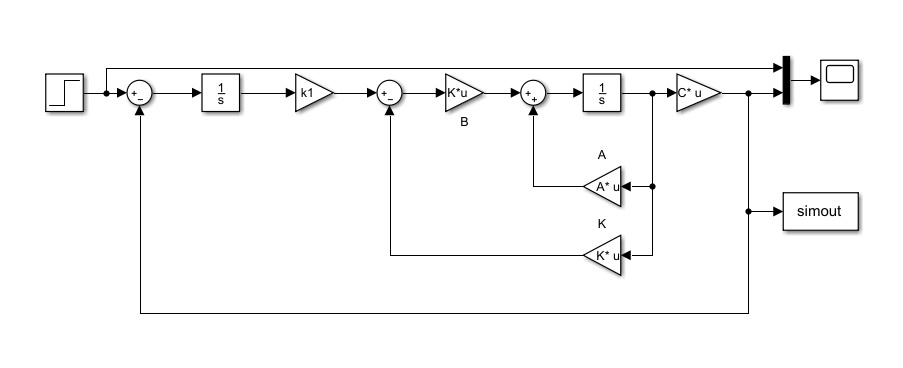
\includegraphics[width=1\linewidth]{stare.png}
	\captionof{figure}{Schema Simulink pentru regulatorul de stare}
	\label{fig:test2}
\end{figure}

Performanțele sistemului de reglare sunt destul de bune, deși pentru obținerea acestora a fost nevoie de mai multe încercări de determinare a polilor sistemului de ordin 2. Deși $M_v$ și $t_s$ 
pentru sistemul de ordinul 2 au valori mai mari decât cele impuse în cerința proiectului, s-a încercat atingerea criteriilor de performanță impuse deoarece cu valorile impuse răspunsul prezenta $t_s=30$. Valorile celui mai bun sistem de regalre dupa stare poate fi observat  în Tab. 6 și Fig. 10.
\begin{center}
	\captionof{table}{Performanțele folosind regulatorul de stare}
	\begin{tabular}{|c|c|c|c|c|c|c|}
		\hline
		&$e_{st}$&$M_v$&$t_s$\\
		\hline
		Impus&0&1&3\\
		\hline
		Obținut&0&1&6.7\\
		\hline
	\end{tabular}
\end{center}

\begin{figure}[H]
	\centering
	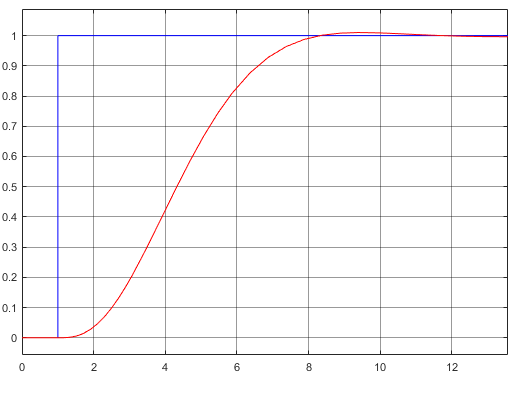
\includegraphics[width=.55\linewidth]{rasp_stare.png}
	\captionof{figure}{Răspunsul sistemului pentru regulatorul de stare}
	\label{fig:test2}
\end{figure}


\section{Concluzii}
Din punct de vedere al ușurinței de proiectare criteriul modului varianta Kessler este cel mai accesibil algoritm. Însă performanțele obținute cu acest regulator nu au îndeplinit cerința timpului de stabilire de 3 secunde sau cea a suprareglajului de 4.56\%. Din acest motiv s-a pornit de la regulatorul PI obținut prin varianta Kessler, s-a adăugat o componentă derivativă pentru a micșora suprareglajul, s-a modificat de asemenea și $T_i$ pentru a reduce timpul de stabilire și s-a ajuns la o performanță foarte apropiată de cea impusă, timpul de stabilire fiind mai lung cu 0.2 secunde.\\
Datorită îndeplinirii criteriilor de performanță, regulatorul obținut prin încercări are și implementare în limbajul C, deși algoritmul propus poate fi aplicat foarte ușor pentru orice ecuație cu diferențe, fiind generic.\\
Pentru metoda experimentală Ziegler-Nichols s-au obținut cele mai slabe performanțe iar metoda de proiectare este relativ dificilă dacă nu avem instrumentele adecvate pentru a determina panta și  pentru a găsi punctul de inflexiune din datele achiziționate. Odată obținute însă valorile $\alpha$ și $L$ se pot încerca diferite tipuri de regulatoare având de făcut niște substituții simple.\\
Regulatorul proiectat după stare a fost cel mai ușor de implementat și testat cu programul Matlab. Singurul impediment este constituit de alegerea polilor conjugați și găsirea unei metode algoritmice de a-i găsi. Metoda aplicată în acest proiect se folosește de forma generală a unui sistem de gradul II și indicatorii de calitate la mărimea de intrare treaptă unitară.  
\newpage

\nocite{*}
\bibliographystyle{ieeetr}
\bibliography{bibliografie}

\end{document}